\chapter{Desarrollo}
\label{chap:desarrollo}
\section{Marco Teorico}
\label{Sec:Marco Teorico Desarrollo}

\subsection{Arquitectura de La U-Net}
\begin{figure}[H]
	\centering
		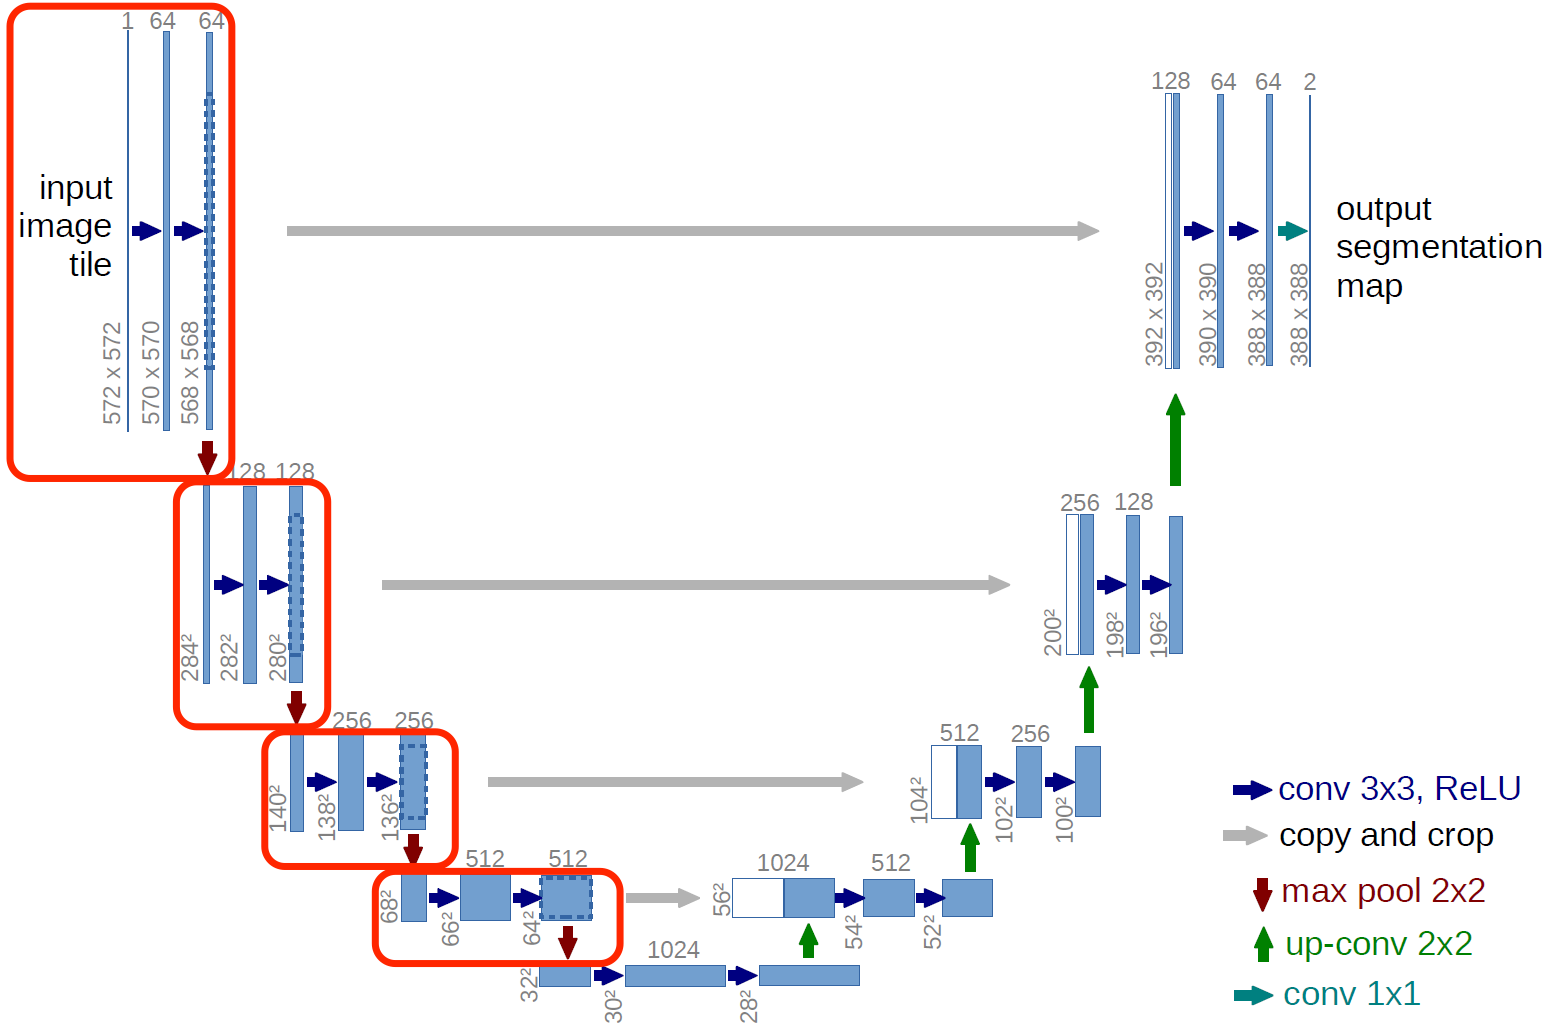
\includegraphics[width=1\textwidth]{06changedetection/unet.png} 
	\caption{Arquitectura original de U-Net}
	\label{fig:ArquitecturaUNET}
\end{figure}

En la \figurename~\ref{fig:ArquitecturaUNET} la arquitectura original de la U-Net~\cite{Ronneberger2015} fue propuesta para imágenes médicas, la U-Net es una red neuronal convolucional realizada para el concurso ``ISBI cell tracking challenge 2015"\footnote{Concurso que consistía en segmentar y rastrear células móviles en secuencias de vídeo.} que consiste en segmentar semánticamente células. La U-Net es caracterizada por que utiliza el copiado de información de las capas de codificación en la sección de decodificación, con esta arquitectura los autores mejoraron los resultados de la segmentación.
La arquitectura comienza con la capa de entrada que es una capa en escala de grises, luego de eso se aplican una serie de convoluciones, la arquitectura tiene 2 partes principales: la de codificación que esta encerrada en rojo y la de decodificación que es el resto. Los tipos de procedimientos usados son:
\begin{itemize}
  \item \textbf{conv 3X3:} Esta es una convolución con filtros de 3 por 3 .
    \item \textbf{copy and crop:} Mediante este proceso se copia la información de las capas codificación en su simétrico de las capas de decodificación.
    \item \textbf{max pool 2x2:} Mediante este proceso se reduce la dimensionalidad de los bloques convolucionales a la mitad para que se pueda procesar mejor.
    \item \textbf{up conv 2x2} Es el proceso para hacer la reconstrucción de la imagen.
\end{itemize}  
La arquitectura propuesta está basada en la U-Net variando las partes del codificador y el decodificador.
\subsection{Bloques residuales}
\label{subsec:residuales}
En el trabajo de \cite{Ruder2016} se presenta el problema de degradación en redes neuronales, este problema se da al aumentar la profundidad la \gls{Accuracy} comienza a bajar. Dicho problema no parece ser natural debido a que si por ejemplo se tiene 2 redes neuronales $a$ y $b$ con $m$ y $n$ capas respectivamente($m$ $>$ $n$), si la red neuronal $a$ utiliza sus $n$ primeras capas de la misma manera que la red $b$, el resto de las capas pueden ser de identidad por la tanto la red neuronal $a$ debería de tener una \gls{Accuracy} por lo menos igual a la red neuronal $b$.  

El problema anterior es resuelto por \cite{Ruder2016} con sus denominados bloques residuales cuya arquitectura esta representado en el siguiente bloque:

\begin{figure}[H]
    \centering
    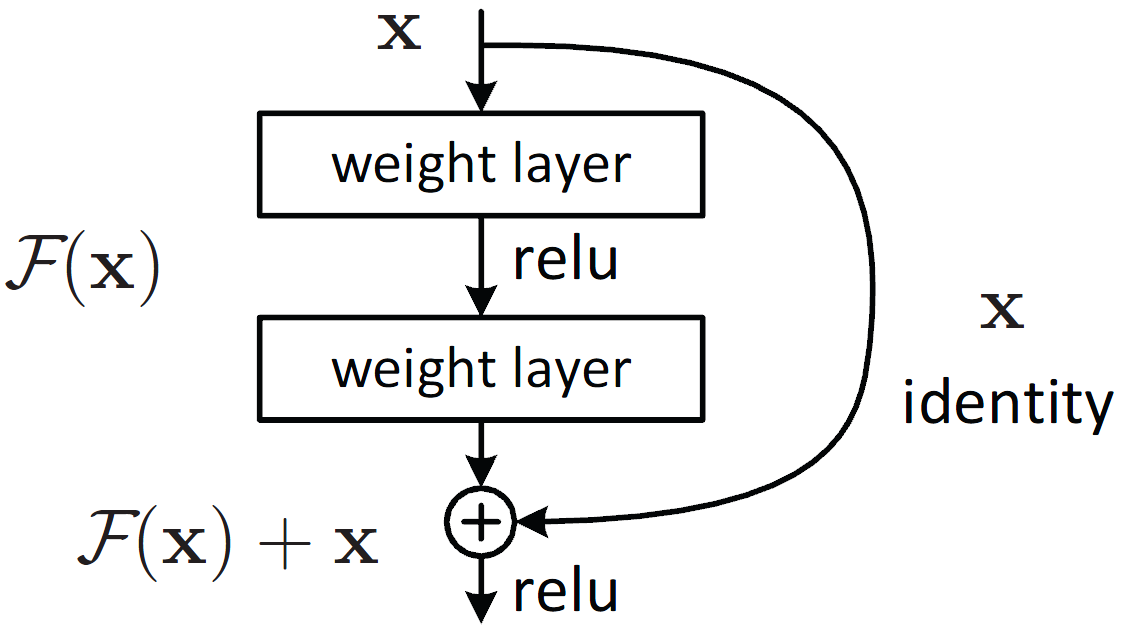
\includegraphics[width =0.7\textwidth]{images/resnet.png}
    \caption{Arquitectura de bloque residual}
    \label{fig:my_label}
\end{figure}


Esta técnica permite a la red neuronal poder transmitir la información de manera más sencilla dado que en caso se necesite la función identidad  los weight layers se asignarían a cero.    
\subsection{Estrategias de partir transformar y mezclar}
Las estrategias de partir transformar y mezclar fueron usados en artículos como \cite{Xie2017, Szegedy2015}, dichas estrategias han demostrado mejorar el rendimiento de las redes neuronal. Por ejemplo \cite{Xie2017} muestra que el uso de estas estrategias lograron una mejora con respecto a sus versiones lineales, esto se aprecia en el siguiente gráfico:
\begin{figure}[H]
    \centering
    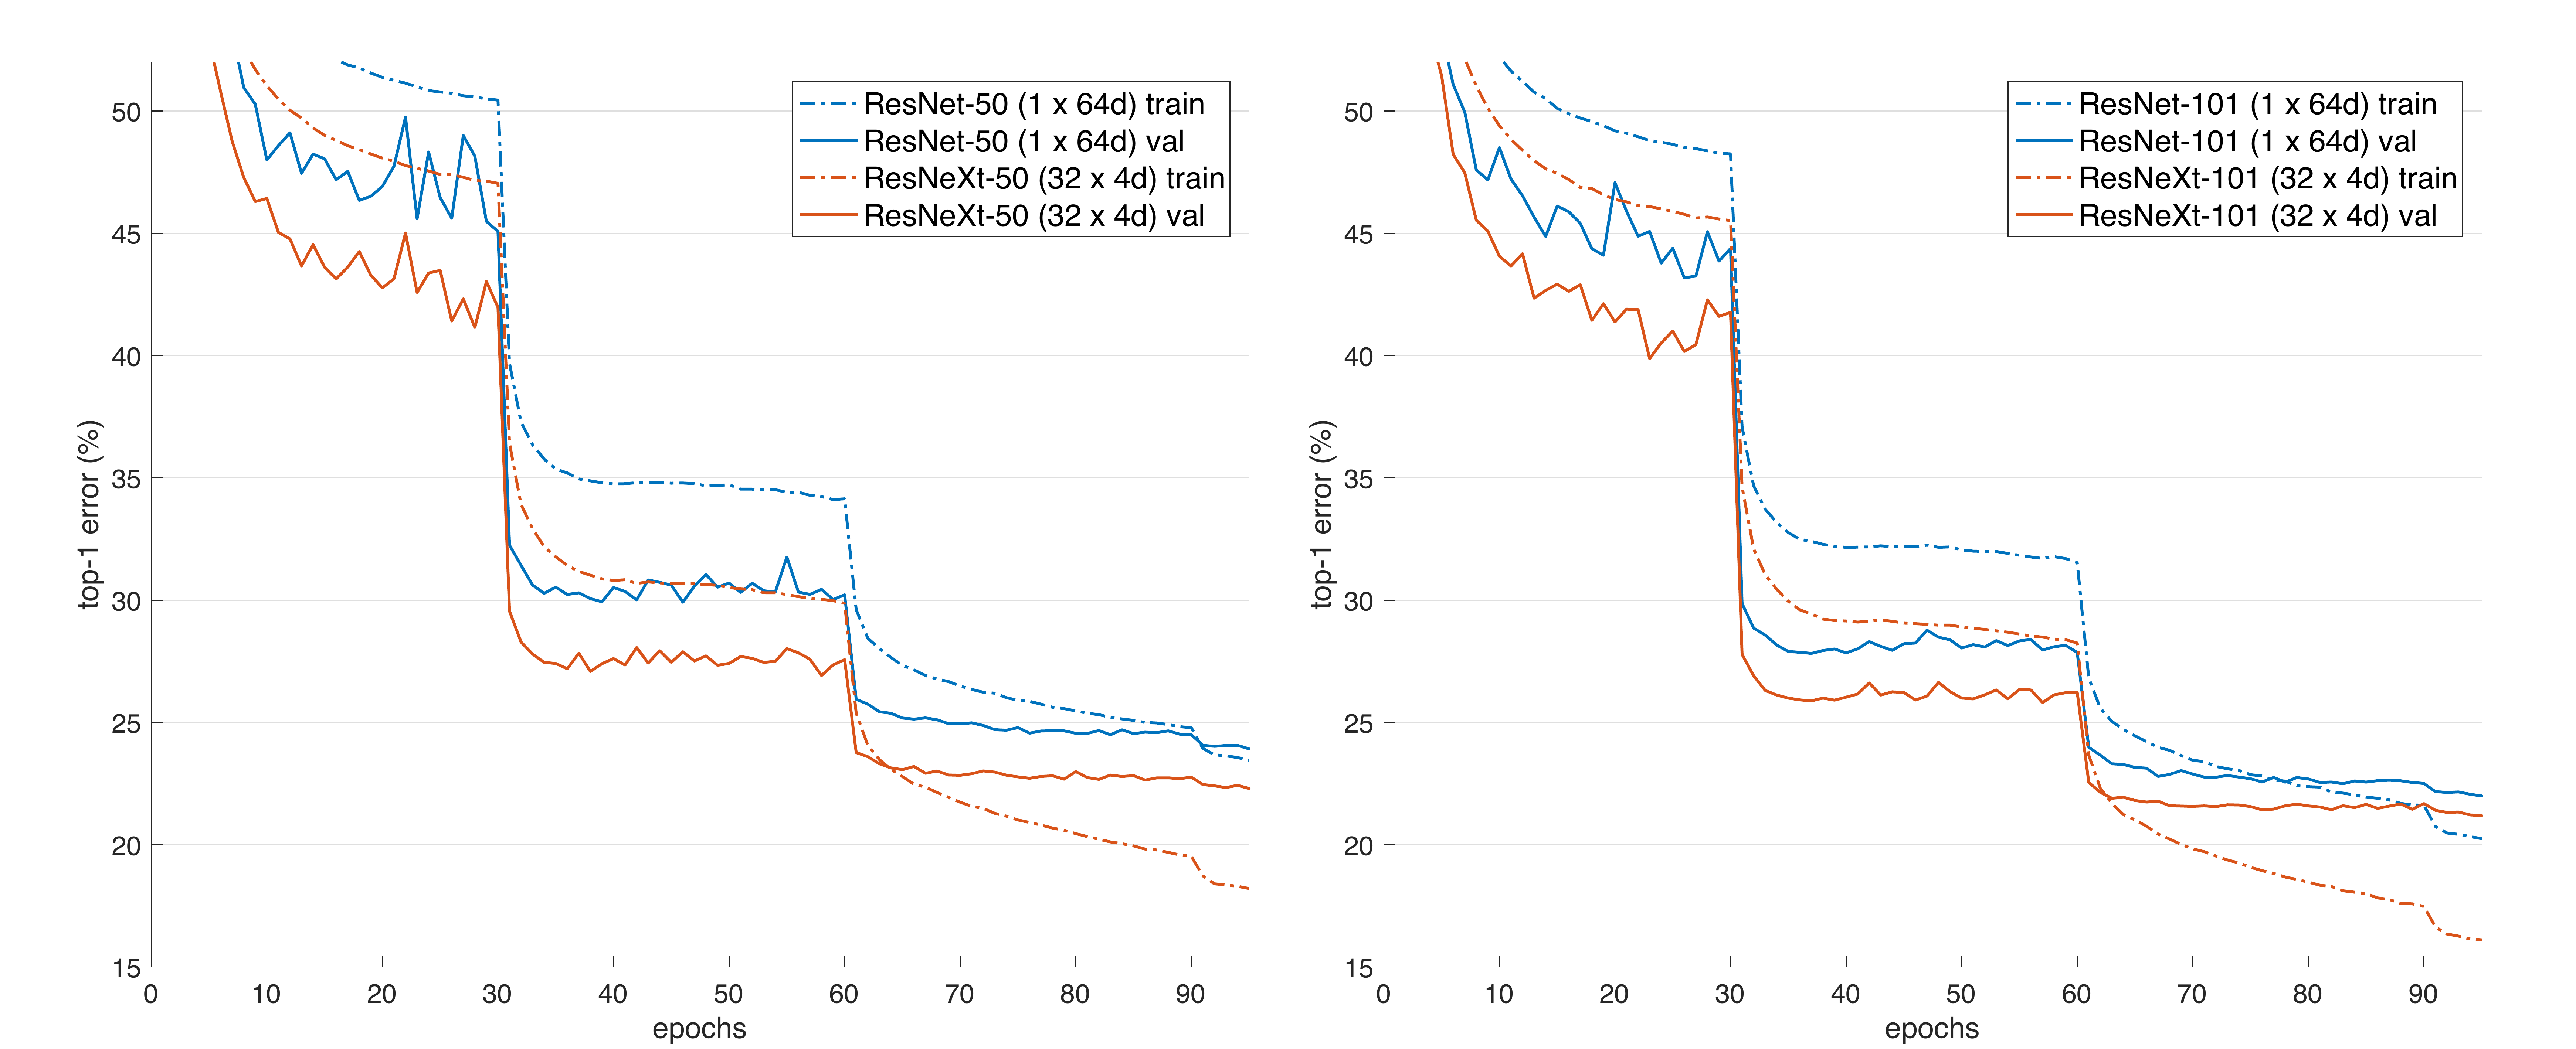
\includegraphics[width=0.9\textwidth]{images/group/resnextMejora.png}
    \caption{Mejora de una Aggregated Transformation propuesta por \cite{Xie2017}}
    \label{fig:mejoraRestnext}
\end{figure}{}
Como se aprecia en la \figurename\ref{fig:mejoraRestnext} el uso de la Aggregated Transformation mejora en alrededor de un 1\% el resultado final, además de acelerar un el proceso de entrenamiento. A continuación se mostraran algunas redes que presentan la estrategia  de partir transformar y mezclar. 
\subsection{Resnext}
\label{subsec:resnext}
La estrategia propuesta por \cite{Xie2017} introduce el concepto de cardinalidad, este concepto para el autor significa la transformación de una convolución en una serie de convoluciones más pequeñas. El siguiente gráfico presenta esa idea: 
\begin{figure}[H]
    \centering
    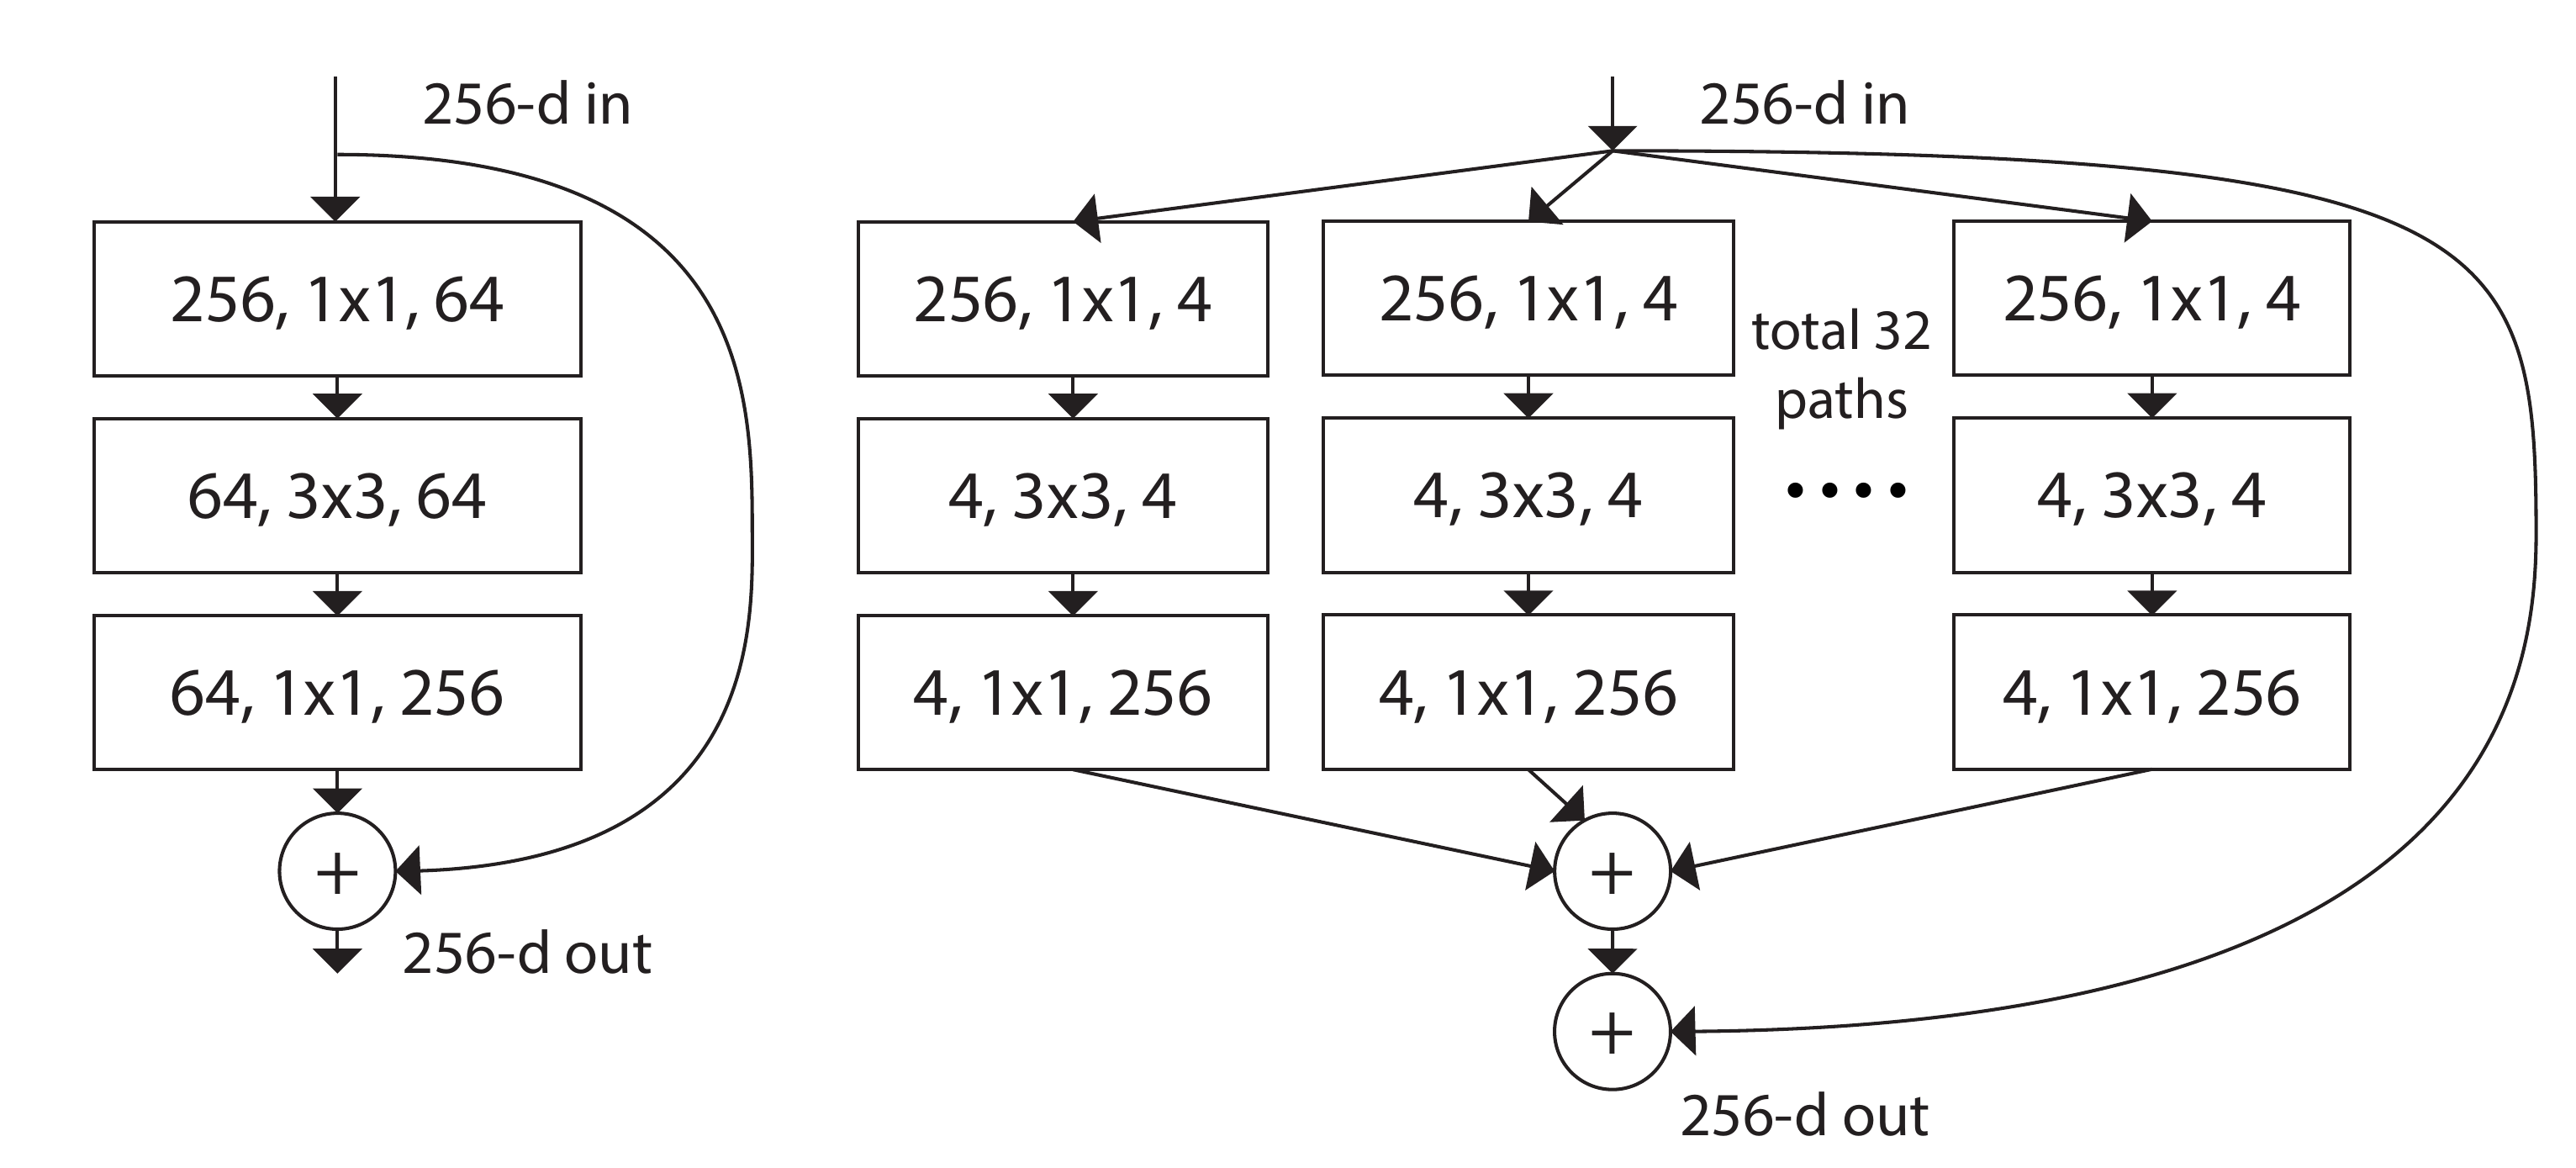
\includegraphics[width= 0.7\textwidth]{images/group/resnext.png}
    \caption{Se muestra el uso de una cardinalidad 32 para el autor propuesto por \cite{Xie2017}}
    \label{fig:resnextBlock}
\end{figure}{}

Como se aprecia en la \figurename \ref{fig:resnextBlock} una series de convoluciones pueden ser transformadas en varias convoluciones más pequeñas, este cambio permite una que estas redes puedan ser operadas en paralelo con más facilidad. 
\subsection{Inception}
La idea de las redes Inception \cite{Szegedy2015} es utilizar múltiples tamaños de filtros para mejorar los resultados, no obstante en este trabajo se demostró que el costo computacional de utilizar múltiples filtros es muy elevada. El autor soluciona este problema utilizando botlenext que es reducir la cantidad de filtros mediante convoluciones 1 x 1, para luego ampliarlas a la cantidad de filtros originales, esto se muestra en la\figurename \ref{fig:inceptionv1} 
\begin{figure}[H]
    \centering
    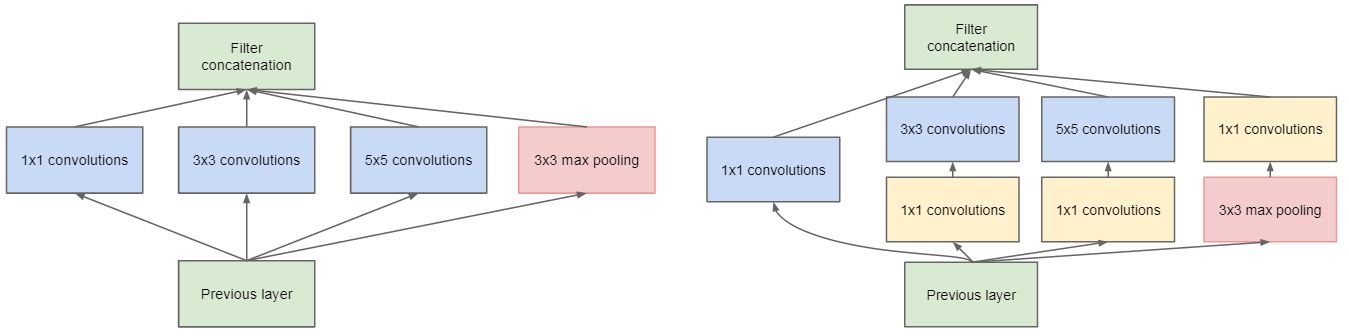
\includegraphics[width= 0.7\textwidth]{images/group/inceptionCortada.png}
    \caption{Arquitectura propuesta en la versión 1 de Google Nets\cite{Szegedy2015}}
    \label{fig:inceptionv1}
\end{figure}{}
Una característica a resaltas de las redes de Google Nets es que cada uno de sus bloques fueron diseñados a comparación de la propuesta de \cite{Xie2017} que se utilizan múltiples bloques iguales.

\subsection{PSP networks}
La Piramid Scene Parsing Networks \cite{zhao2017pyramid} tuvo en consideración el contexto para definir la clasificación de cada pixel, el contexto es obtenido mediante su modulo de conversión piramidal.
\begin{figure}[H]
    \centering
    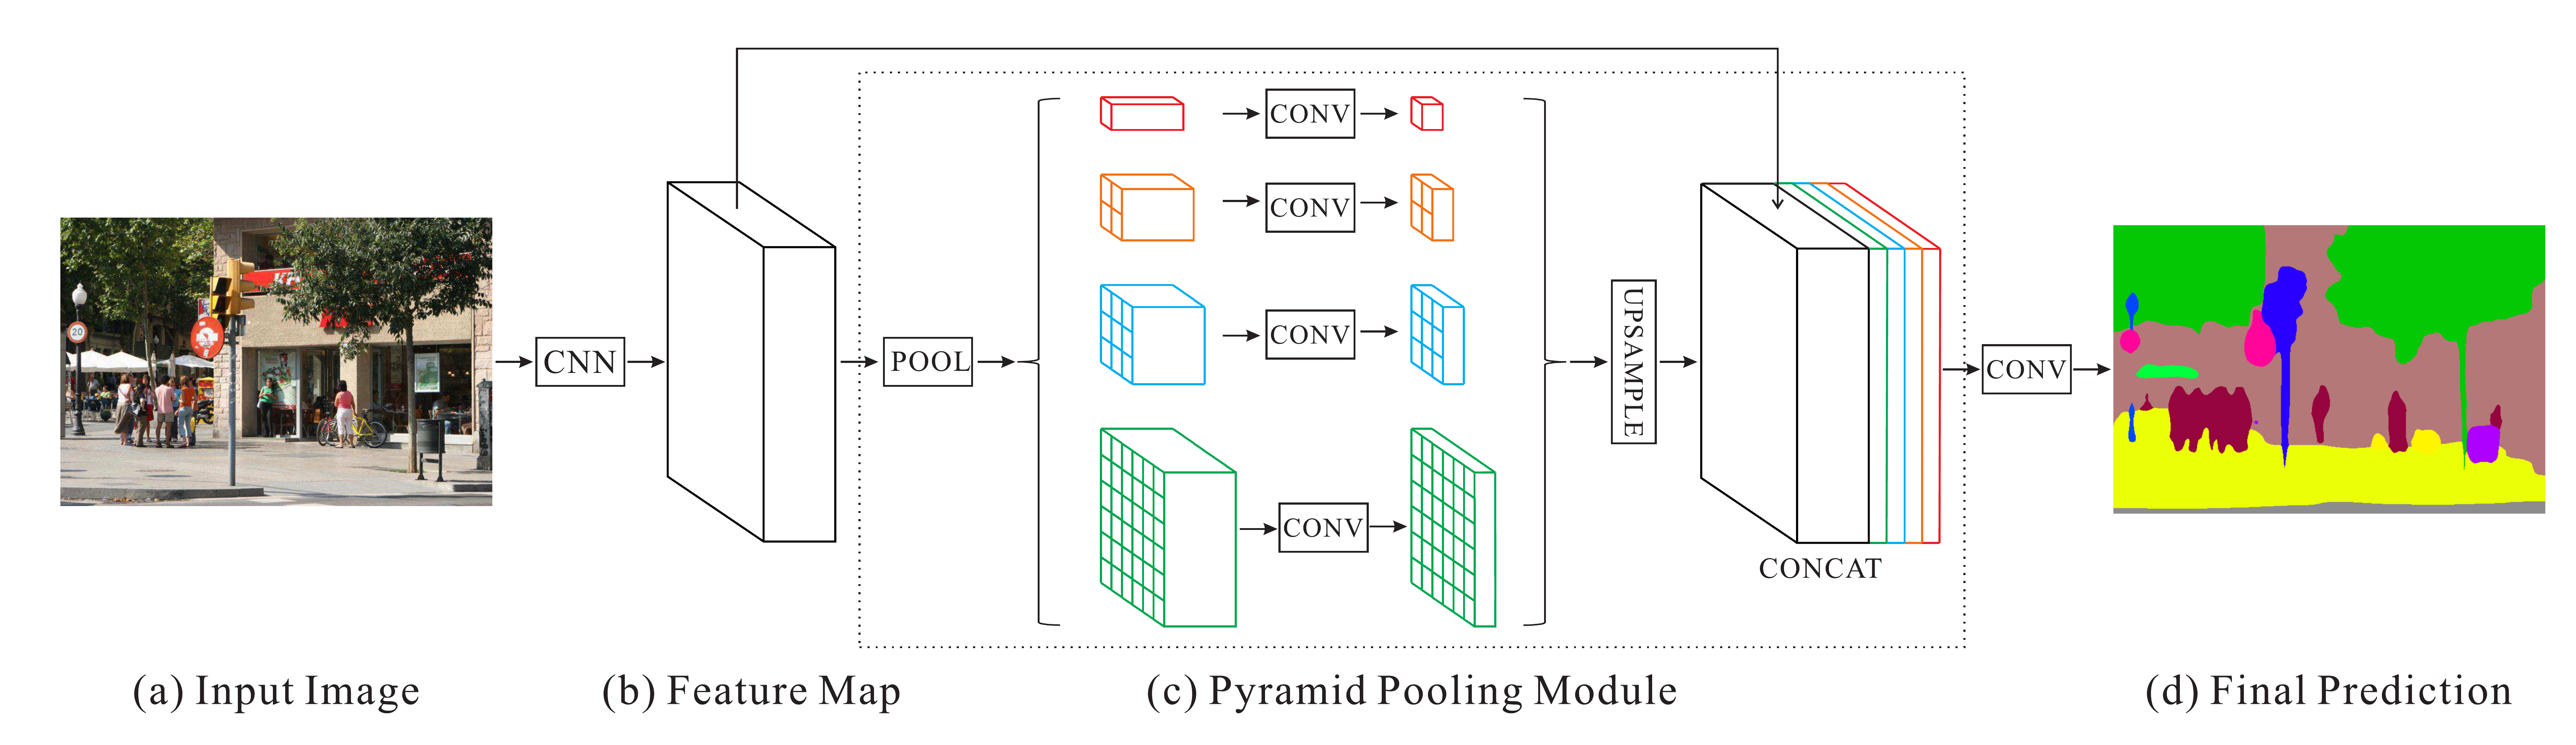
\includegraphics[width = 0.9\textwidth]{images/redes/pspnet.png}
    \caption[Arquitectura PSP]{ Dada una imagen (a), primero se usa una \gls{CNN} para obtener el \gls{Feature Map} para que en la ultimo \gls{Layer}, en (b) el modulo de conversión piramidal es aplicado para obtener distintas representaciones de las subregiones, seguido de un \gls{Upsampling} y concatenación se obtiene el \gls{Feature Map} final, este \gls{Feature Map} porta ambos la información local y la información global contextual. Finalmente el \gls{Feature Map} pasa por unos filtros convolucionales con el fin de obtener un \gls{Layer} por cada clase nesesaria.}
    \label{fig:my_label}
\end{figure}{}
La conversión piramidal se obtiene mediante la aplicación de múltiples tamaños de pooling para que se obtenga la información contextual relacionada a la imagen.

\subsection{Bloque de Squeeze and excitation}
La red convolucional propuesta esta basada en la U-Net, para la parte del codificador se usara una red  basada en el paper de ~\cite{Hu2017} que propone una arquitectura basada en las redes residuales. 
El trabajo propuesto por~\cite{Hu2017} plantea la idea de centrar los esfuerzos de la red en la relación de los canales de un capa convolucional, esto lo hace mediante su técnica de agrupamiento y excitación representada en el siguiente gráfico.
\begin{figure}[H]
	\centering
		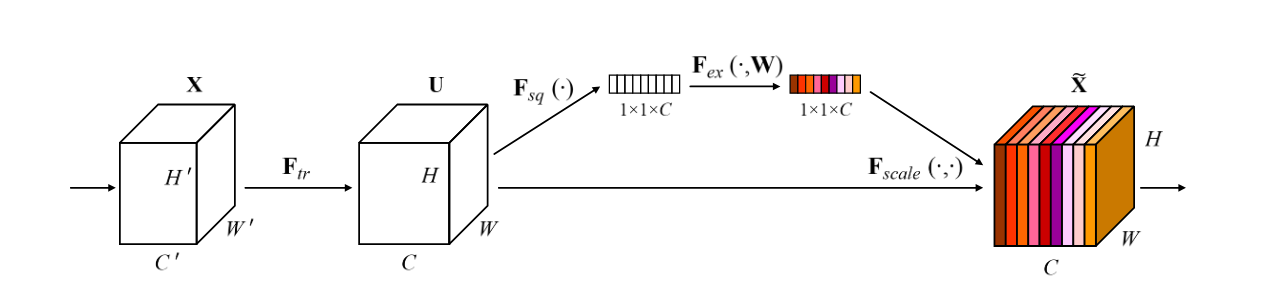
\includegraphics[width=1\textwidth]{06changedetection/SenetBlock.png} 

	\caption[Técnica de agrupamiento y excitación de las SE-Net]{La técnica de agrupamiento y excitación consiste en obtener un valor por cada canal de la capa convolucional luego aplicarle convoluciones al vector resultante para que finalmente los valores obtenidos sean usados como método de  ponderación del bloque convolucional original.}
	\label{fig:Senett}
\end{figure}
En el caso de una red neuronal residual las convoluciones se retransmiten. En el caso de la red neuronal propuesta por~\cite{Hu2017} se procesa un representativo de la capa para poder hacer la convolución correspondiente.

\begin{figure}[H]
	\centering
		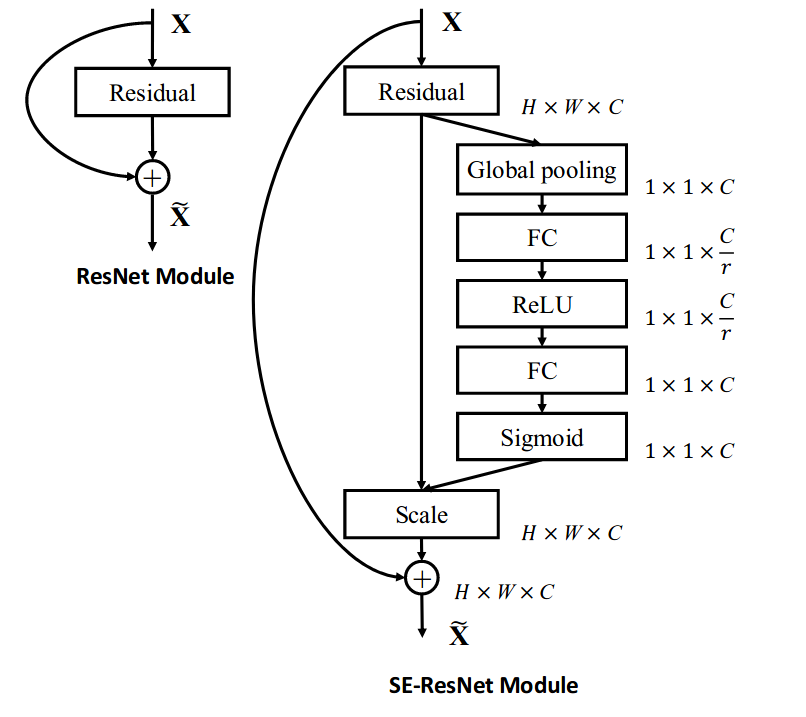
\includegraphics[width=0.7\textwidth]{06changedetection/senet_resnet.png} 
	\caption[Comparación ResNet y Se-Resnet]{Imagen comparativa de una red residual normal vs una red de agrupamiento y excitación.}
	\label{fig:Senett}
\end{figure}


Como se menciona en el trabajo de \cite{Liu2015} el contexto para la segmentación semántica juega un papel muy importante, es por eso que autores como: \cite{Liu2015,Yuan2018 ,zhao2017pyramid} desarrollaron distintas propuestas para incluir el contexto en los procesos de las redes neuronales profundas.



\subsection{Decodificador}

La parte del decodificador esta basada en el trabajo de~\cite{Yuan2018}, este trabajo esta basado en el uso de información del contexto para determinar la clase del píxel, su modulo de obtención de contextos puede ser visto como forma de transformar una capa convolucional en otra con mayor información contextual, este proceso fue nombrado en la implementación del autor como bloque de auto Atención. 

%La formula para el bloque es:
%\begin{equation}
%\label{equ:autoContexto}
%    w_{pi}= softmax(\frac{QK^T}{\sqrt{d_K}})V 
%\end{equation}



La arquitectura propuesta usa la idea de \cite{Yuan2018} como operación antes de generalizar el bloque convolucional con una operación de convolución transpuesta que es demostrada en la siguiente imagen:
\begin{figure}[H]
	\centering
		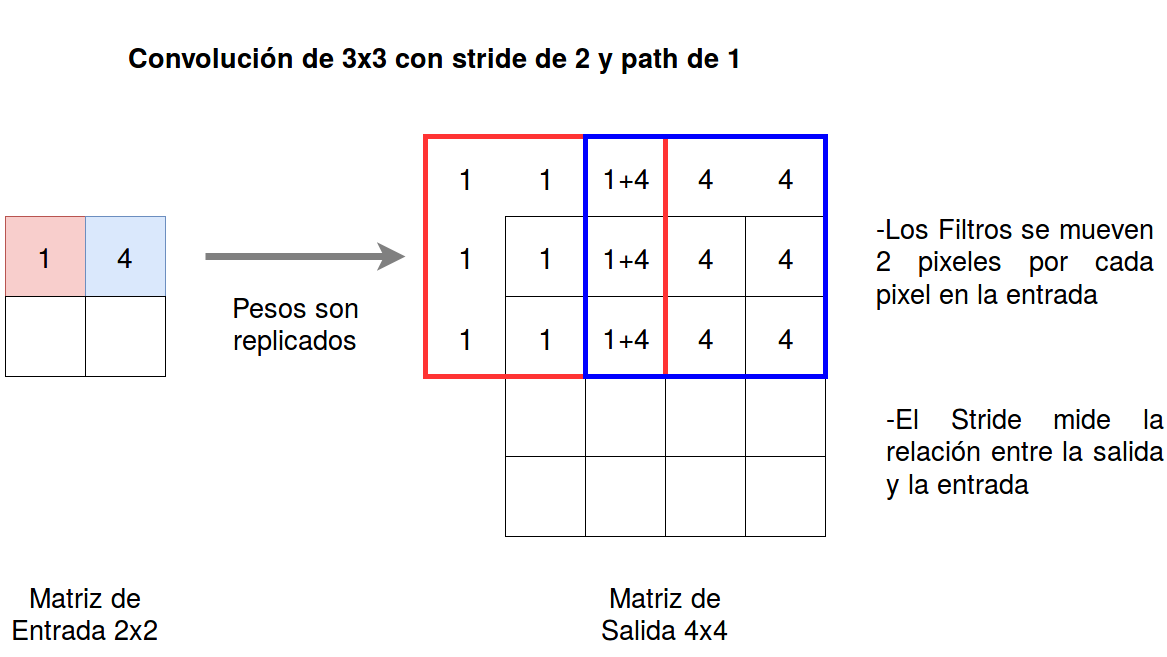
\includegraphics[width=0.7\textwidth]{06changedetection/Transconvolucion.png} 
	
	
	\caption[Procedimiento de una Transconvolución]{Imagen que muestra el procedimiento de una Transconvolución 
}
	\label{fig:Senett}
\end{figure}

\subsection{Función de Perdida }



 La función de perdida usada es la propuesta en el trabajo de \cite{Berman2017} dicha función de perdida  esta basada en el índice de Jaccard descrita previamente en la Sección \ref{section:metricsevaluation} para este trabajo se llamara al índice de Jaccard como \gls{iou}. El autor menciona que su función de perdida fue optimizada para los casos de segmentación semántica.





\subsection{Optimizador}

Se puede considerar a Adam \cite {kingma2014adam}como una combinación de RMSprop y el método de gradiente descendiente con momento. Utiliza las gradientes cuadrados para escalar la velocidad de aprendizaje como RMSprop y aprovecha el momento al usar el promedio móvil del gradiente en lugar del gradiente como SGD con impulso. Adam es un método de tasa de aprendizaje adaptativo, lo que significa que calcula las tasas de aprendizaje individuales para diferentes parámetros. Su nombre se deriva de la estimación del momento adaptativo, y la razón por la que se llama así es porque Adam usa estimaciones del primer y segundo momento del gradiente para adaptar la tasa de aprendizaje para cada peso de la red neuronal.


\section{Descripción de la red neuronal}

\subsection{Bloques utilizados }
\subsubsection{BotleNext}
\begin{figure}[H]
    \centering
    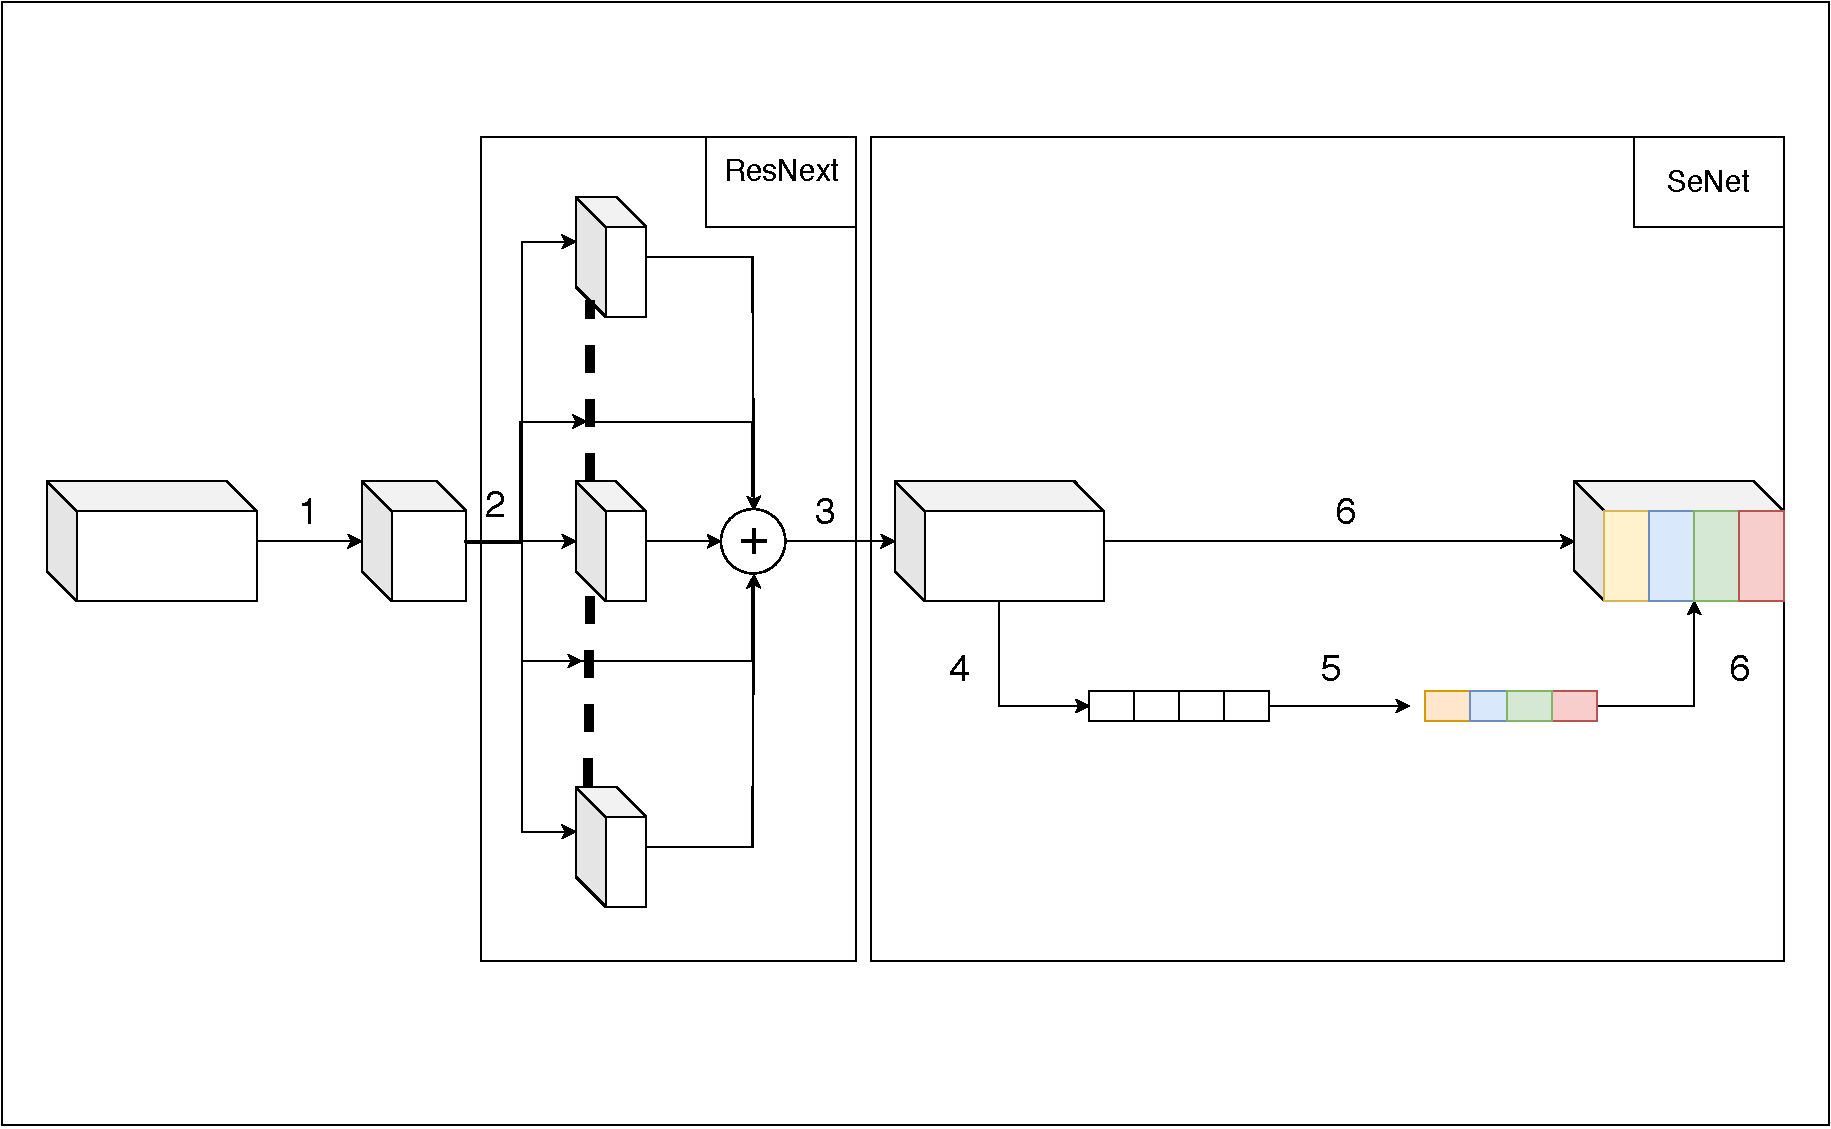
\includegraphics[width=0.9\textwidth]{images/blocks/botlenext.pdf}
    \caption{Modulo Básico del Encoder}
    \label{fig:moduloEncoder}
\end{figure}
Como se aprecia en la figura \ref{fig:moduloEncoder} el modulo básico del encoder es la propuesta en el paper de \cite{Hu2017}, ver la subsección \ref{subsec:residuales} y la subsección \ref{subsec:resnext} 
\begin{enumerate}
    \item  La primera parte es una convolución de 1 x 1 .
    \item  El siguiente modulo es el planteado en la red neuronal ResNext propuesta en el trabajo de \cite{Xie2017}.
    \item  Se pasa a realizar la concatenación de los módulos generados en el paso anterior.
    \item Convolución  de 3 por 3 \label{paso4}
    \item Se comienza con el proceso propuesto por \cite{Hu2017} un adaptative pooling\footnote{El objetivo de este es generar un poling con una salida ya determinada} con resultado final de un solo canal.
    \item Se realiza una convolución 1 x 1.
    \item Se pasa a realizar la multiplicación de cada canal con su respectivo bloque. del bloque obtenido en el paso \ref{paso4} 
\end{enumerate}
\subsubsection{Ocnet Bloque base}
\begin{figure}[H]
    \centering
    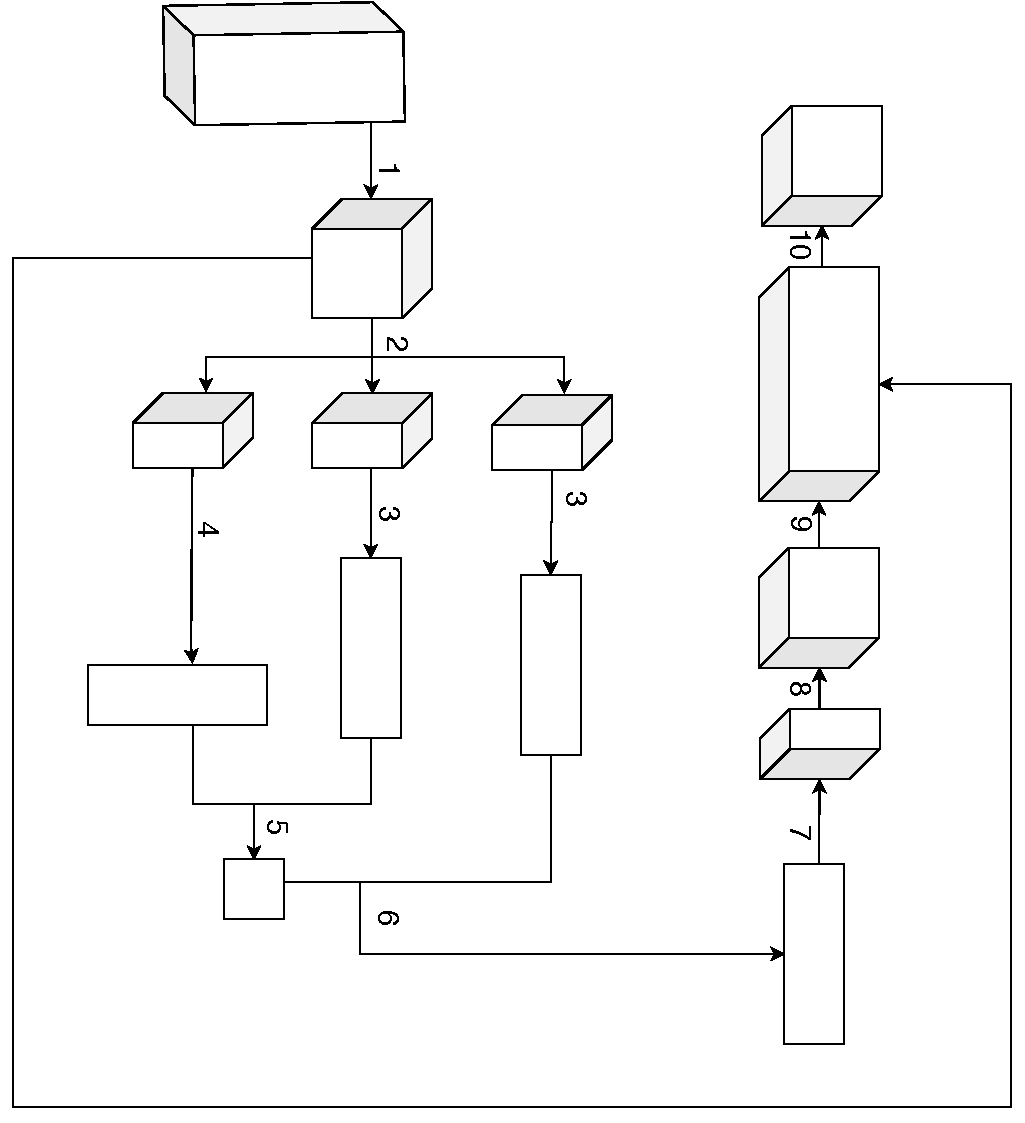
\includegraphics[width=0.8\textwidth]{images/blocks/decoder.pdf}
    \caption{Arquitectura OCBase}
    \label{fig:my_label}
\end{figure}
\begin{enumerate}
    \item Se realiza una convolución para reducir la cantidad de \gls{Layer}s del \gls{Feature Map}
    \item Se reduce aun más la cantidad de \gls{Layer}s para obtener 3 grupos denominados Query, key, Value.
    \item Se reducen las dimensiones de la red neuronal con el fin de poder operar el proceso descrito en el paper de \cite{yuan2018ocnet}.
    \item En este caso ademas de reducir las dimensiones se opera realiza la operación de la trasnpuesta.
    \item Multiplicación del Query con el Key
    \item Multiplicacion del Value con el resultado de 5. 
    \item Se reconstruye la dimensionalidad. 
    \item Se duplica la cantidad de Layers mediante convoluciones 3x3.
    \item  Se duplica la cantidad de Layersconvoluciones 3x3.
    \item Se concatena el valor obtenido en 1 con el valor obtenido en 8.
    \item Se reduce la cantidad de \gls{Layer}s convolucionales mediante convoluciones 1x1.
\end{enumerate}{}

\subsubsection{Logit}
\begin{figure}[H]
    \centering
    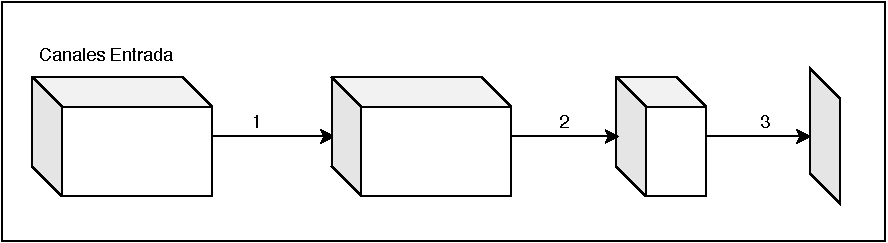
\includegraphics[width = 0.8\textwidth]{images/blocks/logitv2.pdf}
    \caption{Bloque logit}
    \label{fig:my_label}
\end{figure}{}
\begin{enumerate}
    \item Se realiza un Drop Out.
    \item Convoluciones de 3 x3 para obtener un 16 \gls{Layer}s.
    \item Convoluciones de 1x1 para obtener un \gls{Layer}.
\end{enumerate}{}
\subsection{Arquitectura}
\label{Sec:RedPropuesta}
\begin{figure}[H]
    \centering
    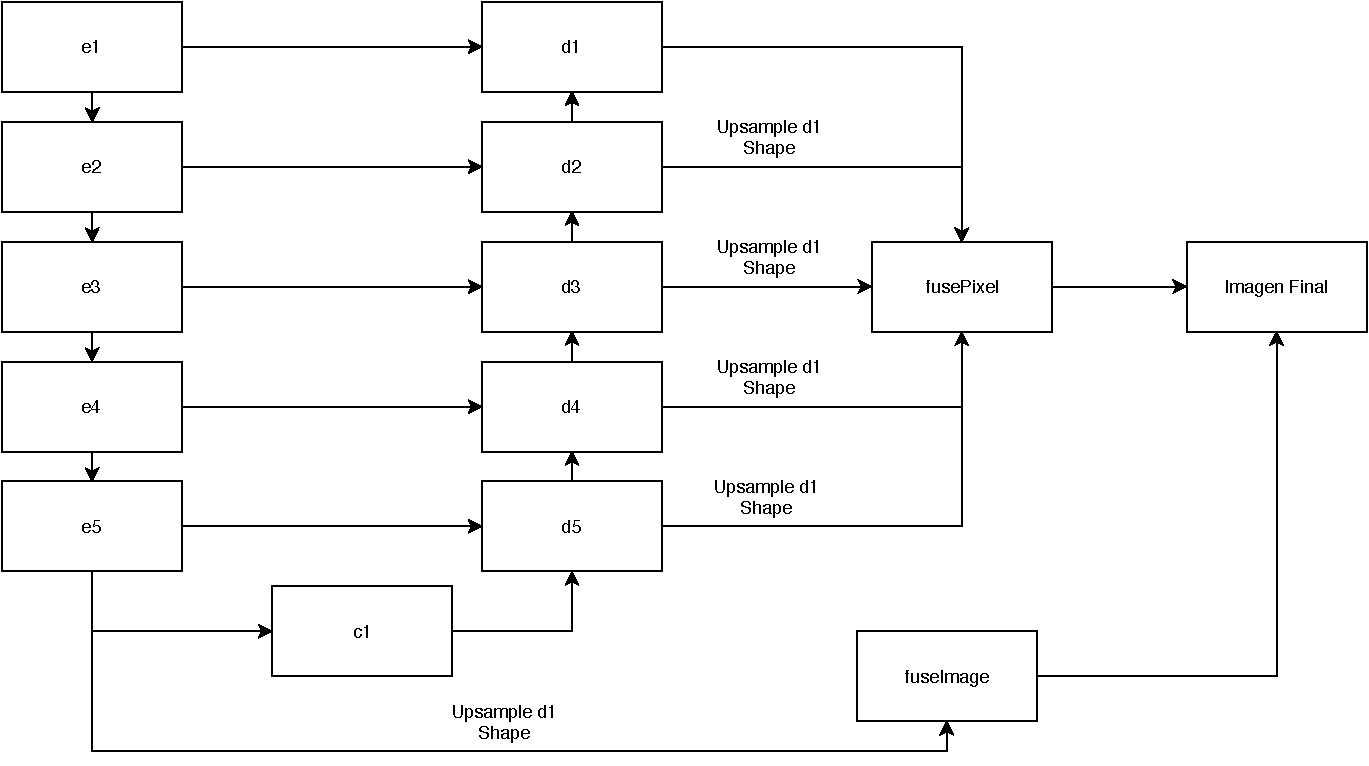
\includegraphics[width=0.8\textwidth]{images/blocks/arquitecturared.pdf}
    \caption{Arquitectura final}
    \label{fig:my_label}
\end{figure}

En esta arquitectura se muestran distintas partes, las descritas en la parte e1,e2,e3,e4,e5  son las partes del encoder, en este proyecto se trabajo con 2 encoders diferentes:
\subsubsection{Encoder Senet-154}
El proceso sera descrito de la siguiente manera 
\begin{enumerate}
    \item \textbf{Entrada-e1}  
       \begin{itemize}
           \item Convolución de 3 x3  con \gls{Stride} 2.
           \item    Normalización por \gls{Batch}es.
            \item    Operación \gls{Relu}.
            \item    convolución d3 3x3 con \gls{Stride}.
           \item    Normalización por \gls{Batch}es.
            \item    Operación \gls{Relu}.
            \item    convolución d3 3x3 con \gls{Stride}.
           \item    Normalización por \gls{Batch}es.
            \item    Operación \gls{Relu}.
       \end{itemize}{}
    \item \textbf{e1-e2:} 1 Bottleneck sin reducción + 3 Bottleneck  sin reducción. 
     \item \textbf{e2-e3:} 1 Botleneck con reducción de Stride 2 + 8 Bottleneck sin reducción. 
     
    \item \textbf{e3-e4:} 1 Botleneck con reducción de Stride 2 + 36 Bottleneck sin reducción.
    \item \textbf{e4-e5:} 1 Botleneck con reducción de Stride 2 + 3 Bottleneck sin reducción.
  %  \item \textbf{e5-c1} 1 Base OCNet module
\end{enumerate}{}
\subsubsection{ Encoder Se-Resnext 51}
El proceso sera descrito de la siguiente manera 
\begin{enumerate}
    \item \textbf{Entrada-e1}  
       \begin{itemize}
        \item Convolución de 3 x3  con \gls{Stride} 2.
           \item    Normalización por \gls{Batch}es.
            \item    Operación \gls{Relu}.
            \item    convolución d3 3x3 con \gls{Stride}.
           \item    Normalización por \gls{Batch}es.
            \item    Operación \gls{Relu}.
            \item    convolución d3 3x3 con \gls{Stride}.
           \item    Normalización por \gls{Batch}es.
            \item    Operación \gls{Relu}.
            
            
            
            
            
       \end{itemize}{}
    \item \textbf{e1-e2:} 1 Bottleneck sin reducción + 3 Bottleneck  sin reducción. 
     \item \textbf{e2-e3:} 1 Botleneck con reducción de Stride 2 + 4 Bottleneck sin reducción. 
     
    \item \textbf{e3-e4:} 1 Botleneck con reducción de Stride 2 + 6 Bottleneck sin reducción.
    \item \textbf{e4-e5:} 1 Botleneck con reducción de Stride 2 + 3 Bottleneck sin reducción.

\end{enumerate}{}
\subsubsection{Decoder}
    \begin{enumerate}
    \item \textbf{e5-c1:} OCNet Bloque Base
    \item \textbf{(c1-e5)-d5:}  Se concatenan los bloques c1 y e5. Luego de esto se  aplica el Bloque Ocnet.
    \item \textbf{(d5-e4)-d4:}  Se concatenan los bloques e4 y d5. Luego de esto se  aplica el Bloque Ocnet.
    \item \textbf{(d4-e3)-d3:}  Se concatenan los bloques e3 y d4. Luego de esto se  aplica el Bloque Ocnet.
    \item \textbf{(d3-e2)-d2:}  Se concatenan los bloques e2 y d3. Luego de esto se  aplica el Bloque Ocnet.
    \item \textbf{(d2-e1)-d1:}  Se concatenan los bloques e1 y d2. Luego de esto se  aplica el Bloque Ocnet.
    


    \end{enumerate}{}


\subsection{Deeplab}
La arquitectura de Deeplab utiliza el concepto de las convoluciones dilatadas mencionada anteriormente en la subsección  \ref{sub:convolucionTranspuesta}.

\begin{figure}[H]
    \centering
    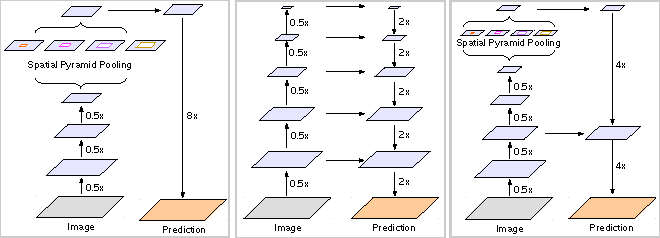
\includegraphics[width = 0.9\textwidth]{images/redes/deeplabv1.pdf}
    \caption{Arquitectura Deeplab obtenida de \cite{Chen2018}}
    \label{fig:deeplabv1}
\end{figure}{}
La imagen a la izquierda muestra la arquitectura propuesta en el trabajo de \cite{zhao2017pyramid} en este modulo se muestra se presenta el Spatial Pyramid Pooling. La parte 2 es una arquitectura parecida a la propuesta en la Unet. La imagen de la derecha muestra la arquitectura propuesta en Deeplabv1 en el cual se utiliza una combinación de las 2 arquitecturas. 

\begin{figure}[H]
    \centering
    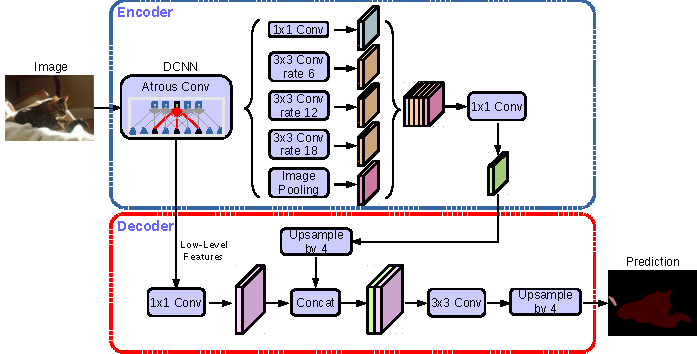
\includegraphics[width = 0.9\textwidth]{images/redes/deeplab.pdf}
    \caption{Arquitectura Deeplab obtenida de \cite{Chen2018}}
    \label{fig:my_label}
\end{figure}{}
En la versión 3 de DeepLab se utiliza el concepto de las convoluciones dilatadas, según las hipótesis del autor de DeepLab v3 la utilización de convoluciones dilatadas provee una segmentación semántica más aguda en los bordes, esto debido a que la convolución dilatada tiene mayor cobertura a medida que se aumentan las convoluciones.



%
\section{Estructura del código fuente}

\begin{center}
    \begin{forest}
 dir tree,
  before drawing tree={
    for tree={
      tikz+/.wrap 2 pgfmath args={\node [anchor=west, font=\footnotesize, text=red] at (.east) {L:#1; n:#2};}{level()}{n()}
    }
  }
 [ Proyecto.
[ datasets.
[ \_\_init\_\_.py.]
[ \_\_pycache\_\_.]
[ salt\_identification.py.
]]
[ Final.py.]
[ fold0-submission.csv.]
[ last-model-fold3.pth.]
[ lastModel.pth.]
[ losses.
[ \_\_init\_\_.py.]
[ lovasz\_losses.py.]
[ \_\_pycache\_\_.]
]
[ mitest.py.]
[ models.
[ basenet.py]
[ \_\_init\_\_.py]]]
\end{forest}
   \newpage

    \begin{forest}
 dir tree,
  before drawing tree={
    for tree={
      tikz+/.wrap 2 pgfmath args={\node [anchor=west, font=\footnotesize, text=red] at (.east) {L:#1; n:#2};}{level()}{n()}
    }
  }
 [ Proyecto.
 [models
[ inplace\_abn]
[ oc\_net.py]
[ \_\_pycache\_\_]
[ unet.py]]
[ mytest]
[ mytrain]
[ probarIOU.py]
[ PruebaEnNotebook.ipynb]
[ README.md]
[ requerimientos.txt]
[ runs
[ fold2
[ checkpoints
[ best-accuracy-checkpoint-fold3.pth]
[ best-loss-checkpoint-fold3.pth]
[ best-metric-checkpoint-fold3.pth]
[ last-checkpoint-fold3.pth]]
]]]
\end{forest}
   \newpage
    \begin{forest}
 dir tree,
  before drawing tree={
    for tree={
      tikz+/.wrap 2 pgfmath args={\node [anchor=west, font=\footnotesize, text=red] at (.east) {L:#1; n:#2};}{level()}{n()}
    }
  } [ Proyecto.
  [ runs
[ fold2
[ models
[  best-accuracy-model-fold3.pth]
[ best-loss-model-fold3.pth]
[ best-metric-model-fold3.pth]
[ last-model-fold3.pth]
][ events.out]
][ fold3]
[ fold4]
][ run.sh]
[ test.py]
[ train.py]
[ transforms]
[ utils]
]
\end{forest}
\end{center}
\section{Descripción de los archivos}
En esta sección se describirá brevemente los archivos del sistema
\subsection{Dataset}
\label{sub:database}
Carpeta contenedora del dataLoader\footnote{Herramienta de soporte para cargar los datos en el modelo} el archivo se llama \textbf{saltidentification.py} a continuación se detalla el contenido de cada archivo.
\begin{itemize}        
    \item \textbf{\_\_init.py\_\_:} En este archivo se usara como medio de importación en otras carpetas
    \item \textbf{saltidentification:} Este archivo contiene la información del dataLoader, aquí se definen los modos con los cuales se carga la data, la direcciones se definen en la función \textbf{load\_images\_and\_masks} el cual retorna un diccionario con los siguientes datos 
    \begin{itemize}
        \item \textbf{mask:}Este dato represente el groundTruth del resultado de la segmentación. Su tipo de dato un arreglo tipo float32.
        \item \textbf{image\_id} El identificador de la imagen a procesar.
        \item \textbf{input} Este dato representa la imagen  a trabajar es un arreglo tipo float32.
        
    \end{itemize}
    
    En la función \textbf{load\_images\_and\_masks} es donde se reduce la imagen de 256x256 a 128x128, además es la función donde se define el umbral de la binarización para el entrenamiento.
\end{itemize}
\subsection{Looses }
Carpeta donde se encuentran definidas distintas funciones de perdida utilizadas en el entrenamiento, el principal archivo de esta carpeta es \textbf{lovasz\_losses.py} en donde se implementa la función de perdida definida en \cite{yu2015lov}.
\subsection{Models}
En este carpeta se define los modelos utilizados para la red neuronal.
\begin{itemize}
    \item \textbf{basenet.py} En este red se encuentran definidos todos los encoders que se pueden utilizar :'vgg11', 'vgg13', 'vgg16', 'vgg19','vgg11 \_bn', 'vgg13 \_bn', 'vgg16 \_bn', 'vgg19 \_bn','resnet18', 'resnet34', 'resnet50', 'resnet101', 'resnet152','resnext101 \_32x4d', 'resnext101 \_64x4d','se \_resnet50', 'se \_resnet101', 'se \_resnet152','se \_resnext50 \_32x4d', 'se \_resnext101 \_32x4d', 'senet154','darknet') , sin embargo las redes que comiensan con VGG tiene un bug, no utilizar.
    \item  \textbf{oc \_net.py} Definición del decoder, esta implementación esta basada en el articulo de \cite{yuan2018ocnet}
    \item \textbf{unet.py} En este archivo se ensambla el encoder con su respectivo decoder creando así el modelo de red neuronal ha utilizar para el entrenamiento
\end{itemize}
\subsection{mytrain}
\label{sub:mytrain}
En esta carpeta se encuentran las imágenes utilizadas para el entrenamiento. Las imágenes en esta carpeta presentan el formato de train\_\textbf{id}.jpg o train\_\textbf{id}.tif donde id representa el identificador de la imagen. Se debe tomar en cuenta que no todas las imagenes en esta carpeta seran utilizadas para el entrenamiento, solamente las imágenes cuyo id este en algún archivo que cumpla la siguiente expresión train\_\textbf{id}.json. 
Cada imagen que cumpla la condición definida en el parrafo anterior debera de contar con una carpeta con el siguiente formato train\_\textbf{id}\_json  en dicha carpeta se tendrá el archivo \textbf{label.png} que es la mascara de la segmentación usada como groundTrue. La generación de los archivos de imágenes se puede hacer con el script \textbf{Listarjson.py}.
\subsection{mytest}
\label{sub:mytest}
En esta carpeta se encuentran los archivos para el testeo de la aplicación, igual que la carpeta mytrain se presenta el mismo formato que lo anterior.

\subsection{PruebaEnNotebooks.ipynb}
Archivo que contiene una presentación de validación de resultados,la funcionalidad de este archivo sera mencionado en la subsección \ref{Avances}
\subsection{runs}
Carpeta que contiene los modelos de entrenamiento, esta carpeta tiene varias subcarpetas que corresponden a cada uno de los entrenamientos hechos anteriormente:

\subsection{corre.sh}
\label{sub:corre}
Este archivo contiene el script necesario para ejecutar el entrenamiento. El contenido del scrip es el siguiente :
\begin{lstlisting}

python train.py --vtf --pretrained imagenet --loss-on-center --batch-size 6 
--optim adamw --learning-rate 8    e-4 --lr-scheduler noam --basenet senet154 
--max-epochs 600 --data-fold fold4 --log-dir runs/fold4 
--resume runs/fold4/checkpoints/last-checkpoint-fold4.pth
\end{lstlisting}
De esto si se desea entrenar de nuevo, es nesesario cambiar de directorio de guardado cambiando fold4 por fold5 u otros.


\subsection{tranforms}
Aquí se encuentran los scripts para el aumento de data y la transformación del numpy a tensores de pytorch.
\subsection{utils}
Diferentes scripts que se utilizan en el entrenamiento, los más importantes  son:
\begin{itemize}
    \item \textbf{Metrics} Aquí se definen las métricas para las gráficas de iou u la otra pixel acurracy.
    \item \textbf{adamw} Se define un optimizador.
\end{itemize}
\subsection{train.py}
Este archivo es el que contiene todo el proceso de entrenamiento.

 